\documentclass[a4paper, 12pt]{article}
\title{Rapport TER}
\author{Yves Appriou, Eva Morton, Sebastian Straut}
\date{\today}
\usepackage{amsmath}
\usepackage{amssymb}
\usepackage{graphicx}

\begin{document}

\maketitle

\tableofcontents.
\newpage.
\section{Introduction}
\begin{figure}
  \begin{center}
    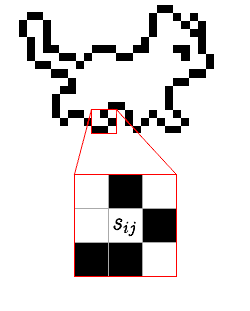
\includegraphics[width=200px]{images/figure1.png}
  \end{center}
  \caption{image 1}
\end{figure}
\section{Définition d'un champ de Markov ?à modifier}
\section{Echantillonnage de réalisations de champs de Markov}
\subsection[Algorithme de Gibbs]{Algorithme de Gibbs}
On s'intéresse maintenant plus en détail à l'algorithme de Gibbs, développé dans les années 1960. Celui-ci se construit de la façon suivante : 
\begin{itemize}
\item On choisit tout d'abord un pixel $s_{ij} $ aléatoirement dans l'image.
\item On calcule ensuite l'énergie locale $U_s(x_0=\lambda_i| \mathcal{V}_s), \forall \lambda_i \in \mathbb{E}$ pour chacun des états possibles. On obtient alors le vecteur des énergies locales suivant : 
\[
  U(x_0) = \left(
          \begin{array}{ll}
            U_s(x_0=\lambda_1| \mathcal{V}_s) \\
            U_s(x_0=\lambda_2| \mathcal{V}_s) \\
            ...\\
            U_s(x_0=\lambda_k| \mathcal{V}_s) \\
          \end{array}
        \right)
\]
\item On produit alors, à partir de cette mesure, une réalisation de la loi de Gibbs : 
\end{itemize}
\[
  \mu = P(x_1 = \lambda) = \frac{1}{Z} \left(
          \begin{array}{ll}
            \exp(-U_s(x_0=\lambda_1| \mathcal{V}_s)) \\
            \exp(-U_s(x_0=\lambda_2| \mathcal{V}_s)) \\
            ...\\
            \exp(-U_s(x_0=\lambda_k| \mathcal{V}_s)) \\
          \end{array}
        \right)
        , Z= \sum_{i\in \mathbb{E}} {U_s(x_1=i | \mathcal{V}_s)}
\]
La probabilité que le site $s_{ij}$ prenne la valeur $\lambda_i$ au temps n+1 est donc donnée par le $i^{\grave{e}me}$ élément du vecteur de la loi de Gibbs.
\begin{itemize}
\item Enfin, on tire dans $\mathbb{E}$ muni de la loi $\mu$, et on remplace par l'état tiré.
\end{itemize}
Pour le modèle d'Ising, par exemple, on a $\mathbb{E} =\{0,1\}$;

\subsection[Algorithme de Metropolis]{Algorithme de Metropolis}
\begin{itemize}
\item On choisit tout d'abord un pixel $s_{ij} $ aléatoirement dans l'image.
\item On récupère l'état du site $s_{ij} $, noté $\lambda_s$ et à valeurs dans $\mathbb{E}$, puis on calcule l'énergie locale du site : 
\[
  U_s(x_0=\lambda_s| \mathcal{V}_s)
\]
\item On tire ensuite un état $\lambda_r \in \mathbb{E}$ muni de $\mathcal{U}$, la loi uniforme sur $\mathbb{E}$.
\item On calcule l'énergie locale du nouveau site $r_{ij}$ après changement d'état : 
\[
  U_r(x_0=\lambda_r| \mathcal{V}_r = \mathcal{V}_s) 
\]
\item On obtient alors la différence des énergies locales : 
\[
  \Delta U = U_r(x_0=\lambda_r| \mathcal{V}_r)-U_s(x_0=\lambda_s| \mathcal{V}_s)
\]
\item Ainsi : 
\begin{enumerate}
  \item Si $\Delta U < 0$, on remplace l'état du site $s_{ij}$ par $\lambda_r$ ;
  \item Sinon, on tire une probabilité p, et si $p < \exp({-\Delta U })$, on accepte le changement de l'état du site $s_{ij}$ par $\lambda_r$.
\end{enumerate}
\end{itemize}

\section{Applications aux algorithmes de restauration d'images}
\subsection[Modèle d'Ising]{Modèle d'Ising}
\subsection[Modèle de Potts]{Modèle de Potts}
\subsection[Algorithme du recuit simulé]{Algorithme du recuit simulé}

\end{document}
